%ten point, letter paper, single column
\documentclass[letterpaper,10pt, onecolumn, draftclsnofoot]{IEEEtran}

\usepackage{graphicx}                                        
\usepackage{amssymb}                                         
\usepackage{amsmath}                                         
\usepackage{amsthm}                                          

\usepackage{alltt}                                           
\usepackage{float}
\usepackage{color}
\usepackage{fancyvrb}
\usepackage{url}

\usepackage{balance}
\usepackage[TABBOTCAP, tight]{subfigure}
\usepackage{enumitem}
\usepackage{pstricks, pst-node}
\usepackage{listings}
\usepackage{tabularx}

\usepackage{geometry}
%0.75 in margin on each side, total of 1.5 in
\geometry{textheight=8.5in, textwidth=6in}
\usepackage{pgfgantt}

%random comment

\newcommand{\cred}[1]{{\color{red}#1}}
\newcommand{\cblue}[1]{{\color{blue}#1}}

\newcommand{\toc}{\tableofcontents}

\usepackage{hyperref}

\def\name{Thomas Albertine}
\title{The Many Faces of Microbial Communities \\\large Senior Design\\Spring Term Final Report\\}
\author{\name, Michael Phelps}


% The following metadata will show up in the PDF properties
 \hypersetup{
   colorlinks = false,
   urlcolor = black,
   pdfauthor = {\name},
   pdfkeywords = {capstone visualization microbiology microbio senior design},
   pdftitle = {Senior Design Project, Visualizing Microbial Communities},
   pdfsubject = {Senior Design Microbiology Visualizations},
   pdfpagemode = UseNone
 }

\lstset{language=python,
                basicstyle=\ttfamily,
                keywordstyle=\color{blue}\ttfamily,
                stringstyle=\color{red}\ttfamily,
                commentstyle=\color{green}\ttfamily,
                morecomment=[l][\color{magenta}]{\#},
				breaklines=true,
				showstringspaces=false
}

\parindent = 0.0 in
\parskip = 0.1 in

%Single space
\linespread{1.0}

\usepackage{fancyvrb}
\usepackage{color}
\usepackage[latin1]{inputenc}


\makeatletter
\def\PY@reset{\let\PY@it=\relax \let\PY@bf=\relax%
    \let\PY@ul=\relax \let\PY@tc=\relax%
    \let\PY@bc=\relax \let\PY@ff=\relax}
\def\PY@tok#1{\csname PY@tok@#1\endcsname}
\def\PY@toks#1+{\ifx\relax#1\empty\else%
    \PY@tok{#1}\expandafter\PY@toks\fi}
\def\PY@do#1{\PY@bc{\PY@tc{\PY@ul{%
    \PY@it{\PY@bf{\PY@ff{#1}}}}}}}
\def\PY#1#2{\PY@reset\PY@toks#1+\relax+\PY@do{#2}}

\expandafter\def\csname PY@tok@gd\endcsname{\def\PY@tc##1{\textcolor[rgb]{0.63,0.00,0.00}{##1}}}
\expandafter\def\csname PY@tok@gu\endcsname{\let\PY@bf=\textbf\def\PY@tc##1{\textcolor[rgb]{0.50,0.00,0.50}{##1}}}
\expandafter\def\csname PY@tok@gt\endcsname{\def\PY@tc##1{\textcolor[rgb]{0.00,0.25,0.82}{##1}}}
\expandafter\def\csname PY@tok@gs\endcsname{\let\PY@bf=\textbf}
\expandafter\def\csname PY@tok@gr\endcsname{\def\PY@tc##1{\textcolor[rgb]{1.00,0.00,0.00}{##1}}}
\expandafter\def\csname PY@tok@cm\endcsname{\let\PY@it=\textit\def\PY@tc##1{\textcolor[rgb]{0.25,0.50,0.50}{##1}}}
\expandafter\def\csname PY@tok@vg\endcsname{\def\PY@tc##1{\textcolor[rgb]{0.10,0.09,0.49}{##1}}}
\expandafter\def\csname PY@tok@m\endcsname{\def\PY@tc##1{\textcolor[rgb]{0.40,0.40,0.40}{##1}}}
\expandafter\def\csname PY@tok@mh\endcsname{\def\PY@tc##1{\textcolor[rgb]{0.40,0.40,0.40}{##1}}}
\expandafter\def\csname PY@tok@go\endcsname{\def\PY@tc##1{\textcolor[rgb]{0.50,0.50,0.50}{##1}}}
\expandafter\def\csname PY@tok@ge\endcsname{\let\PY@it=\textit}
\expandafter\def\csname PY@tok@vc\endcsname{\def\PY@tc##1{\textcolor[rgb]{0.10,0.09,0.49}{##1}}}
\expandafter\def\csname PY@tok@il\endcsname{\def\PY@tc##1{\textcolor[rgb]{0.40,0.40,0.40}{##1}}}
\expandafter\def\csname PY@tok@cs\endcsname{\let\PY@it=\textit\def\PY@tc##1{\textcolor[rgb]{0.25,0.50,0.50}{##1}}}
\expandafter\def\csname PY@tok@cp\endcsname{\def\PY@tc##1{\textcolor[rgb]{0.74,0.48,0.00}{##1}}}
\expandafter\def\csname PY@tok@gi\endcsname{\def\PY@tc##1{\textcolor[rgb]{0.00,0.63,0.00}{##1}}}
\expandafter\def\csname PY@tok@gh\endcsname{\let\PY@bf=\textbf\def\PY@tc##1{\textcolor[rgb]{0.00,0.00,0.50}{##1}}}
\expandafter\def\csname PY@tok@ni\endcsname{\let\PY@bf=\textbf\def\PY@tc##1{\textcolor[rgb]{0.60,0.60,0.60}{##1}}}
\expandafter\def\csname PY@tok@nl\endcsname{\def\PY@tc##1{\textcolor[rgb]{0.63,0.63,0.00}{##1}}}
\expandafter\def\csname PY@tok@nn\endcsname{\let\PY@bf=\textbf\def\PY@tc##1{\textcolor[rgb]{0.00,0.00,1.00}{##1}}}
\expandafter\def\csname PY@tok@no\endcsname{\def\PY@tc##1{\textcolor[rgb]{0.53,0.00,0.00}{##1}}}
\expandafter\def\csname PY@tok@na\endcsname{\def\PY@tc##1{\textcolor[rgb]{0.49,0.56,0.16}{##1}}}
\expandafter\def\csname PY@tok@nb\endcsname{\def\PY@tc##1{\textcolor[rgb]{0.00,0.50,0.00}{##1}}}
\expandafter\def\csname PY@tok@nc\endcsname{\let\PY@bf=\textbf\def\PY@tc##1{\textcolor[rgb]{0.00,0.00,1.00}{##1}}}
\expandafter\def\csname PY@tok@nd\endcsname{\def\PY@tc##1{\textcolor[rgb]{0.67,0.13,1.00}{##1}}}
\expandafter\def\csname PY@tok@ne\endcsname{\let\PY@bf=\textbf\def\PY@tc##1{\textcolor[rgb]{0.82,0.25,0.23}{##1}}}
\expandafter\def\csname PY@tok@nf\endcsname{\def\PY@tc##1{\textcolor[rgb]{0.00,0.00,1.00}{##1}}}
\expandafter\def\csname PY@tok@si\endcsname{\let\PY@bf=\textbf\def\PY@tc##1{\textcolor[rgb]{0.73,0.40,0.53}{##1}}}
\expandafter\def\csname PY@tok@s2\endcsname{\def\PY@tc##1{\textcolor[rgb]{0.73,0.13,0.13}{##1}}}
\expandafter\def\csname PY@tok@vi\endcsname{\def\PY@tc##1{\textcolor[rgb]{0.10,0.09,0.49}{##1}}}
\expandafter\def\csname PY@tok@nt\endcsname{\let\PY@bf=\textbf\def\PY@tc##1{\textcolor[rgb]{0.00,0.50,0.00}{##1}}}
\expandafter\def\csname PY@tok@nv\endcsname{\def\PY@tc##1{\textcolor[rgb]{0.10,0.09,0.49}{##1}}}
\expandafter\def\csname PY@tok@s1\endcsname{\def\PY@tc##1{\textcolor[rgb]{0.73,0.13,0.13}{##1}}}
\expandafter\def\csname PY@tok@sh\endcsname{\def\PY@tc##1{\textcolor[rgb]{0.73,0.13,0.13}{##1}}}
\expandafter\def\csname PY@tok@sc\endcsname{\def\PY@tc##1{\textcolor[rgb]{0.73,0.13,0.13}{##1}}}
\expandafter\def\csname PY@tok@sx\endcsname{\def\PY@tc##1{\textcolor[rgb]{0.00,0.50,0.00}{##1}}}
\expandafter\def\csname PY@tok@bp\endcsname{\def\PY@tc##1{\textcolor[rgb]{0.00,0.50,0.00}{##1}}}
\expandafter\def\csname PY@tok@c1\endcsname{\let\PY@it=\textit\def\PY@tc##1{\textcolor[rgb]{0.25,0.50,0.50}{##1}}}
\expandafter\def\csname PY@tok@kc\endcsname{\let\PY@bf=\textbf\def\PY@tc##1{\textcolor[rgb]{0.00,0.50,0.00}{##1}}}
\expandafter\def\csname PY@tok@c\endcsname{\let\PY@it=\textit\def\PY@tc##1{\textcolor[rgb]{0.25,0.50,0.50}{##1}}}
\expandafter\def\csname PY@tok@mf\endcsname{\def\PY@tc##1{\textcolor[rgb]{0.40,0.40,0.40}{##1}}}
\expandafter\def\csname PY@tok@err\endcsname{\def\PY@bc##1{\setlength{\fboxsep}{0pt}\fcolorbox[rgb]{1.00,0.00,0.00}{1,1,1}{\strut ##1}}}
\expandafter\def\csname PY@tok@kd\endcsname{\let\PY@bf=\textbf\def\PY@tc##1{\textcolor[rgb]{0.00,0.50,0.00}{##1}}}
\expandafter\def\csname PY@tok@ss\endcsname{\def\PY@tc##1{\textcolor[rgb]{0.10,0.09,0.49}{##1}}}
\expandafter\def\csname PY@tok@sr\endcsname{\def\PY@tc##1{\textcolor[rgb]{0.73,0.40,0.53}{##1}}}
\expandafter\def\csname PY@tok@mo\endcsname{\def\PY@tc##1{\textcolor[rgb]{0.40,0.40,0.40}{##1}}}
\expandafter\def\csname PY@tok@kn\endcsname{\let\PY@bf=\textbf\def\PY@tc##1{\textcolor[rgb]{0.00,0.50,0.00}{##1}}}
\expandafter\def\csname PY@tok@mi\endcsname{\def\PY@tc##1{\textcolor[rgb]{0.40,0.40,0.40}{##1}}}
\expandafter\def\csname PY@tok@gp\endcsname{\let\PY@bf=\textbf\def\PY@tc##1{\textcolor[rgb]{0.00,0.00,0.50}{##1}}}
\expandafter\def\csname PY@tok@o\endcsname{\def\PY@tc##1{\textcolor[rgb]{0.40,0.40,0.40}{##1}}}
\expandafter\def\csname PY@tok@kr\endcsname{\let\PY@bf=\textbf\def\PY@tc##1{\textcolor[rgb]{0.00,0.50,0.00}{##1}}}
\expandafter\def\csname PY@tok@s\endcsname{\def\PY@tc##1{\textcolor[rgb]{0.73,0.13,0.13}{##1}}}
\expandafter\def\csname PY@tok@kp\endcsname{\def\PY@tc##1{\textcolor[rgb]{0.00,0.50,0.00}{##1}}}
\expandafter\def\csname PY@tok@w\endcsname{\def\PY@tc##1{\textcolor[rgb]{0.73,0.73,0.73}{##1}}}
\expandafter\def\csname PY@tok@kt\endcsname{\def\PY@tc##1{\textcolor[rgb]{0.69,0.00,0.25}{##1}}}
\expandafter\def\csname PY@tok@ow\endcsname{\let\PY@bf=\textbf\def\PY@tc##1{\textcolor[rgb]{0.67,0.13,1.00}{##1}}}
\expandafter\def\csname PY@tok@sb\endcsname{\def\PY@tc##1{\textcolor[rgb]{0.73,0.13,0.13}{##1}}}
\expandafter\def\csname PY@tok@k\endcsname{\let\PY@bf=\textbf\def\PY@tc##1{\textcolor[rgb]{0.00,0.50,0.00}{##1}}}
\expandafter\def\csname PY@tok@se\endcsname{\let\PY@bf=\textbf\def\PY@tc##1{\textcolor[rgb]{0.73,0.40,0.13}{##1}}}
\expandafter\def\csname PY@tok@sd\endcsname{\let\PY@it=\textit\def\PY@tc##1{\textcolor[rgb]{0.73,0.13,0.13}{##1}}}

\def\PYZbs{\char`\\}
\def\PYZus{\char`\_}
\def\PYZob{\char`\{}
\def\PYZcb{\char`\}}
\def\PYZca{\char`\^}
\def\PYZam{\char`\&}
\def\PYZlt{\char`\<}
\def\PYZgt{\char`\>}
\def\PYZsh{\char`\#}
\def\PYZpc{\char`\%}
\def\PYZdl{\char`\$}
\def\PYZti{\char`\~}
% for compatibility with earlier versions
\def\PYZat{@}
\def\PYZlb{[}
\def\PYZrb{]}
\makeatother


\begin{document}
\maketitle
\section{Abstract}

Our client requested that we create a tool to visualize microbial population data, which would help her in her research. To that end, we've created a tool that can load QIIME OTU files containing population data, represent the relationships in the data via a 3d model of a human, and display the model on the screen in such a way that the user can compare it with those of other samples. The ultimate goal is for this comparison to help the user find patterns that he or she would normally miss. Over the course of the project, we've gained technical skills, such as working with the Qt UI toolkit and the MakeHuman project, as well as non-technical skill such as reading code and working with a client.

\clearpage

\tableofcontents

\section{Introduction}
Our client, Dr. Jenna Lang, a microbiology researcher from University of California Davis requested that we create a tool that she could use to visualize microbial population data as human faces. This tool could potentially help microbiology researchers (as well as those from other fields) find patterns that aren't obvious using existing visualization techniques. 

Currently, the standard visualizations are pie charts or heat maps. Unfortunately, Pie charts aren't effective when there are a large number of categories to represent because there are too many slices. Heat maps on the other hand, while still useful to see patterns, do not make proportions between organisms obvious the way pie charts do. Our tool takes advantage of the human brain's ability to recognize and interpret patterns in faces to visualize data, so users can find new patterns that they would normally miss.

Our team consisted of Thomas Albertine and Michael Phelps. We had no formal roles aside from ``developer'', although generally (but not exclusively) Thomas worked on the backend code, loading data files and generating models, while Michael worked on the frontend code, connecting the backend to a user interface (henceforth referred to as UI). Our client played a hands off role. We spoke with her early in the project to collect requirements and have contacted her to revisit requirements or to keep her aprised of how the project is going, but she generally gave usa lot of freedom regarding how to proceed.

\section{Original Requirements Document}
\begin{figure}[h]
	\begin{ganttchart}[vgrid={*1{black, dotted}}]{1}{21}
		\gantttitle{Initial Gantt Chart in Weeks}{21}\\
		\gantttitlelist{1,...,21}{1}\\
		
		%\ganttbar{Task Name}{start}{end}[name] \\
		%\ganttlink{name1}{name2 defaults to elem1 or the like}
		\ganttbar[name=exploremhuman]{Explore MakeHuman API}{1}{4} \\
		\ganttbar[name=fformats]{Explore File Formats}{1}{2} \\
		\ganttbar[name=lfile]{Load File}{3}{3}\\
		\ganttbar[name=mhumanwrapper]{MakeHuman Wrapper}{5}{8}\\
		\ganttbar[name=ldmodel]{Load and Draw Model}{11}{14}\\
		\ganttbar[name=ui]{Basic UI}{9}{10}\\
		\ganttbar[name=rpsmodel]{Rotate / Pan / Scale Model}{15}{16}\\
		\ganttbar[name=polish]{Polish UI}{17}{21}\\
		\ganttbar[name=expfsprt]{Expand File Type Support}{17}{21}\\
		
		\ganttlink{fformats}{lfile}
		\ganttlink{lfile}{mhumanwrapper}
		\ganttlink{exploremhuman}{mhumanwrapper}
		\ganttlink{mhumanwrapper}{ldmodel}
		\ganttlink{ui}{ldmodel}
		\ganttlink{ui}{polish}
		\ganttlink{ldmodel}{rpsmodel}
		\ganttlink{rpsmodel}{polish}
	\end{ganttchart}
	\caption{This is the original Gantt chart for the project.}
\end{figure}

\subsection{Requirements Document}
The Many Faces of Microbial Communities Project

Team Name: ViewCrobe Software

Members: Thomas Albertine, Michael Phelps

\subsubsection{Introduction}

\paragraph{Purpose}
The theory behind the project is that, since there is a specific portion of the human brain dedicated to processing faces, visualizing microbial data as faces allows users to better compare the complex data. Therefore, the purpose of the project is to provide that functionality in a tool usable primarily by microbiologists, but secondarily by researchers in other disciplines.

\paragraph{Scope}
FaceView will be a user-friendly tool for providing visualizations of microbial population data by representing data as 3d models of humans. Given a supported data file, FaceView will allow the user to select a subset of samples from the file from which to generate models based on a subset of the various populations in the file. After these models are generated, these models will be draw to the screen for comparison by users.

In order to enhance user-friendliness, sample subsets will be relatively small for ease of comparison, while population subsets will be significantly larger to allow for more comprehensive comparisons.

\paragraph{Definitions, Acronyms, and Abbreviations}
\begin{itemize}
	\item Model--In the context of this project, ``model'' refers to a 3 dimensional representation of a human based on a subset of the input data. Since a given model is generated from a sample, in some contexts, the two terms may be interchangeable. 
	\item Sample--In the context of an input file, a sample is a subset of the data representing one population. As an example, a sample may contain the number of colonies and which species they are associated with in a petri dish.
	\item Common Camera Angles--A set of configurations for the observer of a 3d scene that are used often. Such a set would include a front view, a profile view, and a three-quarter view at least.
	\item Visualization Profiles--Data files may include many samples and many organism populations. It may contain more populations than there are supported models or model parameters. Therefore it may become necessary to ignore some samples and some organism populations. Furthermore, the user may want to reassign the model parameter that corresponds to a given organism's population to better emphasize differences in that organism among the samples. However, manually modifying which model parameters correspond to which organisms and which samples should be ignored could be time-consuming to do each time. Therefore it may be expedient to create a profile of these settings, which could be saved and loaded later.
	\item Model Parameters--Values that can be passed in when generating a model in order to influence the outcome. For example, nose length might be a model parameter.
	\item Data Parameters--Values that are read from the data. These can be associated with model parameters to make the visualization reflect the data. For example, the population of E. Coli in a set of samples, which may be tied to the nose length in the finished model.
\end{itemize}

\subsubsection{Bibliography}

[1] ``Data Formats,'' [Online]. Available: \newline http://www.metagenassist.ca/METAGENassist/faces/Docs/Format.jsp. [Accessed 6 November 2015].

[2] ``The Magical Number Seven, Plus or Minus Two: Some Limits on our Capacity for Processing Information,'' Psychological Review, vol. 63, pp. 81-97, 1956. 

\subsubsection{Overall Description}
\paragraph{Product Perspective}

This project interacts with several other components. It reads and interprets supported data file formats. The minimal acceptable set of supported formats includes only the tab separated ``Classic QIIME OTU'' format [1], as it is sufficient for use. Expanding the set of supported file formats is a stretch goal. 

Additionally, we include a UI component to facilitate user interaction. This contains several components.

\begin{itemize}
	\item A screen in which the user will direct the application to a data file, a visualization profile which allows the user to configure which attributes are associated with which model features, and optionally a metadata file, containing groups of samples to aid in selection.
	\item A screen in which thumbnail images of the models will be drawn. This screen would also allow users to add and remove models from a group, and select models to be compared in more detail.
	\item A screen in which the selected models will be drawn. At this point, the user would be able to rotate, pan, and zoom around the models in order to better compare their features.
\end{itemize}

We recognize that certain additional features, while not absolutely necessary for a minimal functional product, would enhance usability, and therefore we add, as stretch goals, shortcuts to certain common camera angles, some way to save and load visualization profiles, and a way to export comparison images. Via our UI, a user from our target user group should be able to use our tool to produce their visualization in 5 minutes  or less with approximately 2 minutes or less of initial instruction. 

\begin{figure}[h]
	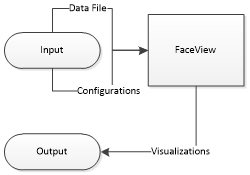
\includegraphics[width=0.4\textwidth]{functional.PNG}
	\caption{A Functional Diagram, demonstrating the interactions between the user and the application.}
	\label{fig:functional}
\end{figure}

\paragraph{Product Functions}
The project should support the following functions

\begin{itemize}
	\item The project should allow the user to select a subset of models to be drawn larger. Note that, in order to allow the user to easily identify similarities and differences in the drawn models, the number of models that can be drawn to the screen, and thus samples that can be represented at once, is limited to 6, since the maximum number of things a person can process at a given time is $7\pm2$ [2].
	\item The project should also support a thumbnail view to select models to view in more detail, and to add and remove models from groups.
	\item Similarly, the project should allow the user to select a subset of organisms to associate with certain module parameters, as those are limited by the number of model parameters that can be modified. 
	\begin{itemize}
		\item Furthermore the user should be able to choose which supported model parameters correspond with which organisms in the data file. This allows the user to allocate more obvious model features to the organisms he or she is most interested in.
	\end{itemize}
	\item The project should, using the data files and visualization profile, generate models and draw them to the screen.
	\item Once these models are drawn to the screen, the user should be able to rotate, pan, and zoom the views. The thumbnail view is exempt from this requirement, as that would make initial screening difficult.
\end{itemize}

\paragraph{User Characteristics}
Our intended users are researchers who are analyzing population data, specifically microbial population data. Such users are highly educated, but do not want to have to use unnecessarily complex or difficult tools.

\paragraph{Assumptions and Dependencies}
We assume that Windows will be installed on the machine running the project. We also assume a version of Python 3 is included.

\subsubsection{Specific Requirements}

\paragraph{Sample Subset}
The project should allow users to select a subset of at most 6 samples to compare in detail. This is to improve user-friendliness. Restricting the number of models shown may reduce distractions, allowing users to better compare certain samples. 

\paragraph{Grouping}
The project should allow users to organize samples into groups for easy profiling of features or comparing subsets of the data. Users should be able to add or remove samples from a given group.

\paragraph{Organism Subset}
The project should allow users to select a subset of organism appearing in the samples. This subset is limited by the number of model parameters which we can support, which should be at least 150. 

\paragraph{Model Parameter Assignment}
The project should allow users to specify certain model parameters to correspond to certain measurements in the data file, such as the population of a certain microbe corresponding to eye shape. This is to improve user-friendliness by allowing users to match parameters used in an existing result, or to allow certain features to be made more obvious.

\paragraph{Classic QIIME OTU Format Support}
Initially, the project should support the tab separated ``Classic'' QIIME OUT format for data files. It is human readable as it looks like a table when viewed in a text editor, which makes it a good choice for a proof of concept. Expanding file format support is a stretch goal. 

\paragraph{Transforming Data}
The project should transform the data from the data file into a format that can be used to generate the models. This allows us to produce a standard format for model generation, which allows us to expand supported file formats.

\paragraph{Producing a Model}
The project should produce a 3d human model based on the parameters from each selected sample. For each model generated in the batch, the same data parameter corresponds to the same model parameter. For example, if the population of a certain microbe in a certain sample corresponded to the straightness of the produced model's nose for that sample, then the population of the same microbe in a second sample would correspond to the straightness of its model's nose. This process should not take longer than 30 seconds.

\paragraph{Drawing Models}
The project should draw the produced models to the screen such that each of the models are viewable at the same time. This is to facilitate the user comparing models.

\paragraph{User Controls}
The project should allow users to rotate, pan, and zoom around the models in order to better compare them. All models should rotate, pan, and zoom.

\subsubsection{Additional ``Stretch'' Goals}

\paragraph{Provide a Web UI}
In addition to the local version, this would provide a web UI which would invoke the component that generates models on the server. These models would then be sent to the client browser to be presented to the user. This stretch goal would necessitate that the project be portable enough to run on a Linux server. 

\paragraph{Export Images for Later Comparison}
This feature would allow users to not only compare samples in the same file, but also to compare to files compared earlier. However, this would allow the user the opportunity to associate different data parameters with different model parameters between the two results, which could lead to misleading results.

\paragraph{Save and Load Visualization Profiles}
This feature would allow users to save and load visualization profiles, configurations of which samples and organisms from a given file are to be used when generating the model, and which organism corresponds to which feature.

\subsubsection{A -- An Explanation of Prerequisites Apparent in the Preliminary Gantt Chart}
\begin{itemize}
	\item Exploring File Formats -- This is time dedicated to choosing a data file type and understanding how to interpret one of those files. It has no dependencies.
	\item Explore MakeHuman API -- This is time dedicated to learning how to use the MakeHuman project to create Human Models programmatically. It has no dependencies
	\item Load File -- This task is to write code to load a data file, and translate it into a standard format. Its prerequisite is to understand a file format.
	\item MakeHuman Wrapper -- This task is to write a wrapper around the MakeHuman project so that we can send the parameters included in the standard parameter format into the project to generate a model. Its prerequisites are to explore the MakeHuman project and to generate the set of standard parameters.
	\item Basic UI -- This task is to create a basic UI through which the user will interact with the other components. Obviously, this will need to be connected to those components so one will be a prerequisite of the other. However, this one has no prerequisites because we need to be able to start somewhere.
	\item Load and Draw Model -- This task is to be able to load and draw a model generated by the MakeHuman project. It's prerequisite is a UI to draw it in.
	\item Rotate, Pan, Scale Model -- This task is to be able to apply the specified transformations to the model, allowing the user to better examine it. It's prerequisite is to be able to load and draw the models.
	\item Expand File Type Support -- This stretch goal is to support more file types. As it is a stretch goal, we would not work on it until we have satisfied the rest of the goals, therefore its prerequisite is to be finished with the rest of the project, represented in the Gantt chart as tasks that are otherwise at the end of a prerequisite chain.
	\item Polish UI -- This stretch goal is to make general cosmetic and user friendliness related improvements to the UI. As another stretch goal, its prerequisites are the same as the other's.
\end{itemize}

\section{Final Requirements Document}
\subsection{Requirements Document Changes}
\begin{center}
	\begin{tabularx}{\textwidth}{|c|X|X|X|}
		\hline
		& Requirement & Change & Comments \\
		\hline
		1 & Assumptions and Dependencies:...We also assume a version of Python 3 is included. & Change Python 3 to Python 2.7 & As it turned out, Makehuman, which we were using to generate the models, only works with versions of Python 2.\\
		\hline
		2 & Organism Subset: The project should allow users to select a subset of organism appearing in the samples. This subset is limited by the number of model parameters which we can support, which should be at least 150. & Changed requirement from 150 model features to 138 & The current version of MakeHuman only supports 138 facial parameters. We could have expanded to other parts of the body, but our client requested faces only.\\ 
		\hline
		3 &  User Controls: The project should allow users to rotate, pan, and zoom around the models in order to better compare them. All models should rotate, pan, and zoom. & Removed zoom and pan & Since all of the parameters were in the face and the camera was already centered on the face, zooming and panning provided little benefit and made the controls unnecessarily complicated.\\
		\hline
	\end{tabularx}
\end{center}

\subsection{Final Gantt Chart}
\begin{figure}[h!]
	\begin{ganttchart}[vgrid={*1{black, dotted}}]{1}{30}
		\gantttitle{Final Gantt Chart in Weeks}{30}\\
		\gantttitlelist{1,...,30}{1}\\
		
		%\ganttbar{Task Name}{start}{end}[name] \\
		%\ganttlink{name1}{name2 defaults to elem1 or the like}
		
		\ganttbar[name=xMH]{A}{4}{4} \\
		\ganttbar[name=xFF]{B}{4}{4} \\
		\ganttbar[name=mHWrapper]{C}{11}{14} \\
		\ganttbar[name=loadDF]{D}{12}{14} \\
		\ganttbar[name=cGrouping]{E}{17}{17} \\
		\ganttbar[name=cOBJ]{F}{18}{19} \\
		\ganttbar[name=cUI]{G}{15}{19} \\
		\ganttbar[name=uUI]{H}{21}{26} \\
		\ganttbar[name=tUI]{I}{20}{20} \\
		\ganttbar[name=mOBJ]{J}{24}{24}
		
		\ganttlink{xMH}{mHWrapper}
		\ganttlink{xFF}{loadDF}
		\ganttlink{mHWrapper}{cOBJ}
		\ganttlink{loadDF}{cOBJ}
		\ganttlink{loadDF}{cGrouping}
		\ganttlink{cUI}{tUI}
		\ganttlink{cOBJ}{tUI}
		\ganttlink{tUI}{uUI}
		\ganttlink{tUI}{mOBJ}
	\end{ganttchart}
	\begin{tabular}{|c|c|}
		\hline
		Entry & Description \\
		\hline
		\hline
		A & Explore MakeHuman API (Tech Review) \\
		\hline
		B & Explore File Formats (Tech Review) \\
		\hline
		C & Create MakeHuman Wrapper \\
		\hline
		D & Load Data File \\
		\hline
		E & Create Grouping Functionality \\
		\hline
		F & Create Obj viewer widget \\
		\hline
		G & Create Initial UI \\
		\hline
		H & Implement UI suggestions\\
		\hline
		I & Test UI \\
		\hline
		J & Extend Obj viewer feature support\\
		\hline
		
	\end{tabular}
	\caption{This is a Gantt chart that more accurately reflects the work on the project. It shows weeks 1 through 30, 10 for each term, since we didn't work on the project on vacation, or during finals week. It does not include time spent working on documentation throughout the term, unless the documentation was related to one of the tasks on the initial chart.}
\end{figure}
\pagebreak

\section{Design Document}
\subsection{Introduction}
\subsubsection{Identification Information}
November 19, 2015 (v0.1)

ViewCrobe Software

Thomas Albertine, Michael Phelps

\subsubsection{Change History}
v0.1 --November 23, 2015

\subsubsection{Purpose}
This document describes the design of the FaceView project. Different components are intended for different audiences, but all will be helpful for the developers creating the project. For stakeholders representing users, the UI and use case sections will be most helpful.

\subsubsection{Scope}
Our goal for the FaceView project is to make it easy to visualize population data as faces. Specifically, such data would be microbial population data, but the same principles apply to many kinds of population data, so the project has applications outside that specific area. These kinds of visualizations may help scientists identify patterns between samples that would otherwise be missed when examined through existing visualization techniques.

\subsubsection{Overview}
This document covers the design from different views. It begins with views more relevant to stakeholders representing users, and moves to additional views that might be more helpful to developers who would need to read the whole document anyway. Within this framework, focus moves from a high level downward when applicable.

In this document, we recognize two stakeholders. Firstly, there are our users. This category also includes the project proposer, as Dr. Lang is a microbiologist and therefore is representative of our primary users. We recognize the following concerns on behalf of our users.

\begin{itemize}
	\item Loading data and file type support
	\item Interpreting data
	\item Viewing results
	\item Large (hundreds of samples) input support
	\item Ease of use
\end{itemize}

Our second stakeholder is the developers of the project. On behalf of our developers, we recognize the following additional concerns.

\begin{itemize}
	\item Maintainability
	\item Interactions between components
\end{itemize}

\subsection{User-oriented Views}
\subsubsection{Use Cases}
The following use cases describe the operations that the FaceView software will support. Depending on the complexity of the use case, commentary may also be included. It behaves as a context viewpoint and addresses user related concerns regarding loading and interpreting data, viewing results, and working with large data sets. We believe that this viewpoint can best describe the general functionality of the product.

\begin{figure}[h]
	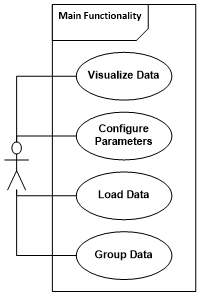
\includegraphics[width=0.4\textwidth]{UseCases.PNG}
	\caption{The four main use cases}
	\label{fig:usecases}
\end{figure}

\subsubsection{Visualize Data}
The obvious goal when using the FaceView visualization software is to visualize the population data. To actually display the visualization, the software must generate a 3d model representing the sample and draw that to the screen. In order to examine all of the aspects of that model, it is necessary to allow users to manipulate that model, so simple transformations are necessary, such as camera rotation, zoom, and pan.

\subsubsection{Load Data}
In order to generate models based on population data, the program must be capable of loading the data. As per our client's request, the project will support, at minimum, the QIIME [1] tab delineated format, as it is well established in the community. It is currently a stretch goal to expand support to other types, such as the BIOM [1] format (which is JSON based) or to a plain CSV format [1].

Additionally, some formats, including QIIME tab delineated may include a metadata file that would allow for categorization. This would be loaded as well.
\subsubsection{Group Data}
In order to handle large data sets, it may be useful to categorize certain selections of samples. As mentioned in the ``Load Data'' section, that initial category data may be loaded from a metadata file, or it may not contain any categories. In either case, categories can be modified later on.

\subsubsection{UI Mockup}
The following is a wireframe mockup of the UI which will clarify how the user will interact with the program. It describes the process for loading a file, the thumbnail view, and the analysis view.

\subsubsection{Load Menu}
\begin{figure}[h]
	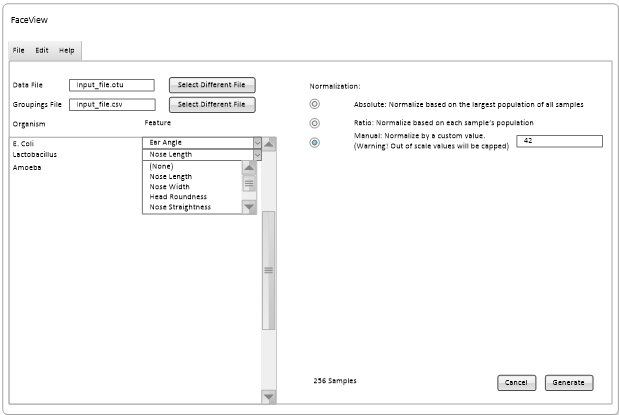
\includegraphics[width=\textwidth]{loadMenu.PNG}
	\caption{A mockup of the UI for loading a file containing three organisms and 256 samples, to be normalized with a maximum value of 42}
	\label{fig:loadingmockup}
\end{figure}

Figure \ref{fig:loadingmockup} is a mockup of the UI for loading an input file and setting parameters. The first step in loading a data file is to select which files to load. The file selection boxes are in the upper left corner. Once files are loaded, the next step is to configure model generation parameters, so dialogs for those parameters are adjacent to the file selection boxes. Finally, the last step is to actually generate the models, so the ``Generate'' and ``Cancel'' buttons are in the lower right, farthest away from the file selection boxes. In this way, the order in which details are specified mimics the order in which the user might interact with other familiar systems, like reading a book.

On the left, the user can specify which model features correspond to which organisms in the data file. That way, users can assign the most interesting organisms to the most interesting features, or prevent uninteresting organisms from being visualized at all. Additionally, this allows users to resolve issues arising from the data file having more organisms than there are model features.

On the right, the user has normalization options. These are important because the range of a population in a data file could be very large, but the model generator only needs to know how pronounced a feature is. This range constraint restricts model parameters from 0, where the feature is nonexistent or minimal, to 1, where the feature is the most pronounced that it can be. In the mockup there are three options for normalization. 

First, there is the option to normalize based on the greatest population of this organism in the file. This allows users to compare populations between samples in the file, which is helpful for drawing conclusions involving the total populations.

Second, there is the option to normalize based on the total population in the sample. This is good if the samples are of varying size, or if the user is more interested in the proportion of the population that is a given organism.

Finally, there is the option to normalize manually based on an arbitrary value. This is convenient if the user wants to compare features to an exported image of a previous sample, but does not want to add it to the existing file, or if the user does not have the data or parameters that were used to generate the existing visualization. 

In the bottom right, there are the ``Cancel'' and ``Generate'' buttons, as well as a count of the number of samples. The two buttons are fairly obvious, but the count is particularly helpful because it allows users to confirm that FaceView was able to correctly read the data file by comparing that number with the expected number of samples. For additional confirmation, the user can compare the organisms found in the organism-model feature association dialog with the expected organisms in the file. 

\subsubsection{Thumbnail View}
\begin{figure}[h]
	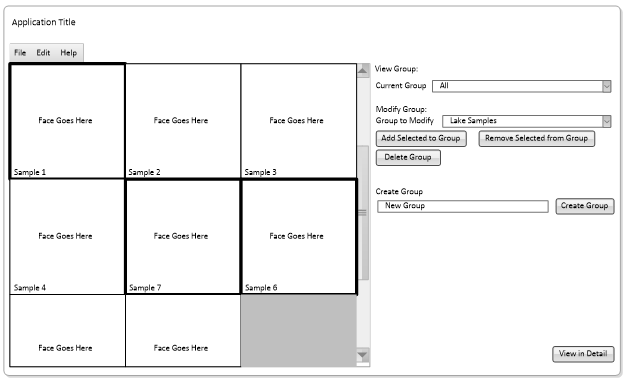
\includegraphics[width=\textwidth]{thumbnailMenu.PNG}
	\caption{A mockup of a Thumbnail View containing eight samples, currently view the group of all samples}
	\label{fig:thumbnailMockup}
\end{figure}

Figure \ref{fig:thumbnailMockup} is a mockup of the thumbnail view. This view allows users to modify groups, filter by groups, and view selected samples in detail. In the mockup, two sections are apparent. The left panel allows users to select, deselect, and preview samples, while the right panel allows users to perform operations on the selection.

The right panel allows the user to specify which group he or she would like to view, add or remove samples from any group, delete a group, or create a new group with the selected elements. There are a few special groups, for the user's convenience. 

The first special group is the ``All'' group. This group is available by default and always contains all samples. Therefore, it cannot be deleted or modified and it will not be selectable on the ``Modify Group'' drop down. The second special group is the ``Selected'' group, which includes only the samples that are currently selected. As viewing models in detail imposes certain constraints described later on, this view is helpful to deselect samples that violate those constraints.

Finally, there is a button to view the samples in detail. The main constraint to view samples in detail is that the user cannot view more than six samples at a time. This is because humans can't keep more than seven plus or minus two things in working memory at any given time [1], so comparing more than seven samples is, in general, more detrimental to users' ability to compare samples. We choose six as the limit, because decreasing the number would make the software slightly more easy to use, and because seven (as a prime number) would result in wasted screen space. This is because it is impossible to arrange seven rectangular objects of the same shape in a two dimensional grid with more than one entry in both dimensions, without leaving empty space.

\subsubsection{Analysis View}
\begin{figure}[h]
	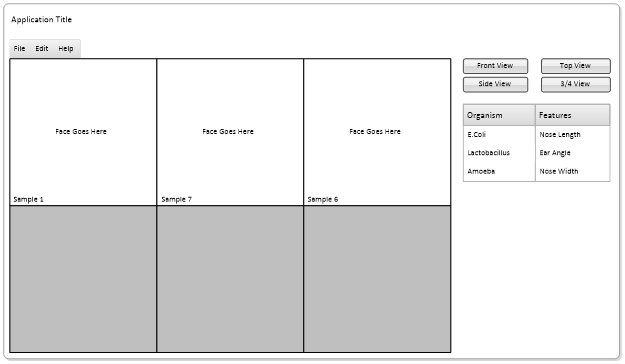
\includegraphics[width=\textwidth]{analysisMenu.PNG}
	\caption{The analysis view, where the selected samples were Sample 1, Sample 7, and Sample 6. If more samples were selected, the three empty windows would be populated.}
	\label{fig:analysisMockup}
\end{figure}

The Analysis View allows user to compare their models more closely. In this view, samples are rendered in 3d in real time, so that users can manipulate them to better compare features. The supported manipulations are camera pan, zoom, and rotate. For ease of comparison, each window is manipulated together. In the event that the user loses the model, perhaps through excessive zooming or panning, there are buttons to return the camera to one of several common camera positions. On the right, next to the camera position buttons, there is a table reminding the user which attributes correspond to which organism. While the mockup only demonstrates three samples, the application supports up to six.

\subsection{Developer-oriented Views}
\subsubsection{General Structure}
\begin{figure}[h]
	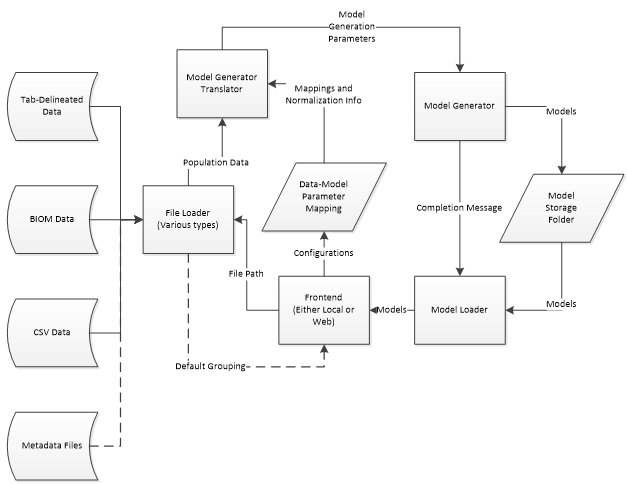
\includegraphics[width=\textwidth]{structure.PNG}
	\caption{A flowchart representing the general structure of the project.}
	\label{fig:structure}
\end{figure}

Figure \ref{fig:structure} summarizes the general structure of the project. It contains each entity in the project as well as their communications (and relationships). The main components of this diagram are the File Loaders, the Model Generator Translator, Data-Model Parameter Mapping, Frontend, Model Generator, and Model Loader.

The entities are presented in the order in which they are invoked in a typical use case, with the exception of the Frontend, which is invoked both at the beginning and the end of the process. These components are likely to be developed in the same order, again, with the exception of the Frontend, as it is easily mocked up for development purposes

\subsubsection{Local Frontend}
The Frontend is where the user instigates any action of the rest of the program. It tells the File Loaders which files to load and when, and it stores the user's Data-Model Parameter Mappings (which also includes normalization settings). When model generation is done, is receives the generated models and thumbnail images from the Model Loader and presents them to the user. It is also where Grouping information is managed, and therefore is where the File Loader sends default grouping information. For more information on the Local Frontend, see UI Mockup. As a stretch goal, we may also create a Web UI so that the tool can be used online. This component will likely be written last, as it depends on a large number of other components, and it can be mocked up and automated for development purposes relatively easily.

\subsubsection{File Loader}
The File Loader is the component that reads files from the filesystem. It is composed of one file type specific loader for each file type (i.e. a BIOM loader) that is registered with a file extension. When a file is passed to the loader with that extension, the loader sends it to the appropriate specific loader, which loads the data. Each specific loader puts the data into a unified format for simplicity later on. This unified data is passed to the Model Generator Translator. 

\subsubsection{Data-Model Parameter Mapping}
The data-Model Parameter Mapping is a structure that contains associations between organisms present in the data and features present in the model. This is configurable by the user between initial file loading and model generation. These configurations are then used in the process of translating population data to model generation instructions. The advantage of this strategy is that, by passing these associations, users can force particular organisms to use more obvious model features. In addition to specifying a feature, there is an option to associate an organism with no feature, in which case it will be ignored, or with any feature, in which case an unallocated feature (or no feature, if none are available) will be chosen for it when it passes through the translator. Users are not guaranteed that the same organisms will be assigned the same features, but the Data-Model associations (including post translation) are listed in the Analysis View described in the UI Mockup section. Normalization configurations are stored in this component as well.

\subsubsection{Model Generator Translator}

The Model Generator translator receives the population data and the Data-Model Parameter Mapping data and uses these to produce instructions for the Model Generator. Though the diagram shows this component interacting directly with the Model Generator, in reality these instructions are passed back to the UI before invoking the Model Generator so that the progress of the visualization process can be presented to the user. It is during this step that the Model Storage Folder is cleaned out, in order to minimize disk space usage.

\subsubsection{Model Loader}
Once the last instance of the Model Generator has terminated, the Model Loader loads the thumbnails on behalf of the Frontend. When the user has selected samples to examine more closely, the Model Loader also loads the obj file human models into a pyopengl-friendly structure. These structures are returned to the Frontend, where they are presented to the user.

\subsubsection{Inter-component Communications}
Most components communicate with each other in a standard way. That is, the return value of the function implementing the component is passed to the next. However, communication between the Model Generator Translator and the Model Generator, communication between the Model Generator and the Model Loader, and communication of the Data-Model Parameter Mappings between the Frontend and the Model Generator Translator do not follow this pattern completely.

\subsubsection{The General Case}
For most communications between components, the process is simple. When the component is invoked, it is contained within a function call. The communication is as simple as the arguments passed in and the return value.

\subsubsection{Model Generator Translator and Model Generator}
The communication between the Model Generator Translator and the Model translator is special because the Model Generator should allow for parallelism. Additionally, it should be independent from the rest of the program, so that it can be easily reused for the Web UI stretch goal. 

To that effect the Model Generator Translator outputs its results as a set of attribute-number pairs, where each attribute is a possible feature of the model, and the number is between zero and one, representing the value or the parameter in terms of its minimum and maximum values. Each sample corresponds to one invocation the Model Generator, which receives the message through stdin. 

\subsubsection{Model Generator and Model Loader}
Since the Model Generator is a special case, as described in the previous section, it communicates the results in a special way as well.
Since the Model Generator can run as a standalone program, it notifies the invoking program that it is finished just like any other child process. The generated models are saved to a folder along with a thumbnail image. Once the Model Generator processes terminate, the Loader can be invoked to load the tumbnails or models.

\subsection{Appendices}
\subsubsection{Glossary}
\begin{itemize}
	\item Model--In the context of this project, a model is a three dimensional representation of the geometry of an object. The project will generate models of faces with facial features representing the data from the input file. For storage purposes, our model geometry is kept in Wavefront obj format.
	\item Transformation--Transformations are operations that can be applied to a point to move it somewhere else. In the project, the camera transformations (which move the vertices that make up a model's geometry to create the illusion that the viewer is moving) will support pan (moving the camera to the side), rotate (turning the camera), and zoom (moving the camera forward and backward, or modifying the camera's field of view).
	\item Normalization--Scaling a set of scalar values so that they all fall in a range between zero and one. In this project, zero corresponds to the minimum a feature can be, while one corresponds to the maximum a feature can be.
	\item CSV--Stands for comma separated value. It is a file format in which fields for a record are separated by a character (often a comma) that does not occur in the data itself, and different records are separated by a different character (often a newline) that also does not occur in the data.
\end{itemize}

\subsection{Citations}
[1] ``Python,'' [Online]. Available: https://www.python.org/. [Accessed 4 November 2015].

[2] ``The Magical Number Seven, Plus or Minus Two: Some Limits on our Capacity for Processing Information,'' Psychological Review, vol. 63, pp. 81-97, 1956. 

[3] ``MakeHuman,'' [Online]. Available: https://bitbucket.org/MakeHuman/. [Accessed 3 November 2015].


\subsubsection{Changes}
There were relatively few changes. The user interface did not match up precisely with the mockup in this document, although it was fairly similar. Additionally, zoom and pan functionality was removed, as it did not provide signficant benefit, and it complicated the controls. We did not update the design document, because the UI changes were trivial, and because the zoom and pan functionality change was late enough that our priority was to ensure that everything was functioning for expo.

Additionally, when writing this document, we overlooked the usefulness of going back one menu, and we added that later as well, so it was not added to this document either, for the same reason as the change regarding zoom and pan functionality.


\section{Tech Review}
Team 36, ViewCrobe Software

Product Name: FaceView

The Many Faces of Microbial Communities

The purpose of this project is to develop software which will allow users to input files containing sample data of microbial communities, and receive human model outputs based on the data within each sample. This mean that our program must accept some form of accepted, preferably common, file type for microbial sample data. It must also be able to convert this data into a data format suitable for our method of facial generation. It must then be able to generate a face based on various input values and output that face as some form of model. 

\subsection{Model Generation}
\subsubsection{MakeHuman}
MakeHuman is a computer graphics software which allows users to create 3D human models through the use of a series of Blender scripts. One of the biggest benefits of MakeHuman is that it is open source with a very unrestricting license which allow it to be free used with commercial and non-commercial projects. This allows us to have control over every aspect of the technology without having to spend time creating our own scripts. MakeHuman also has an in depth API which allows for easy creation and exporting of models based on various criteria. It has proved itself as a high quality project when it was awarded the Suzanne Award for best Blender Python script in 2004. The primary foreseeable downside for MakeHuman is the potential difficulties of utilizing the API in our own software. Overall however, MakeHuman is a well-rounded project with a very clear method utilization, making it a great potential choice for our project.

\subsubsection{Fuse Character Creator}

The second possible technology which could be used is the Fuse Character Creator. The Fuse Character Creator is a computer graphics software developed by Mixamo which allows the creation of 3D character models. The software is mainly designed for use by video game developers and the like. Overall, the models have great detail and could even be considered more realistic than the MakeHuman models. Fuse Character Creator also allows for users to easily import external user generated content, which could potentially be utilized in our project. Unfortunately, Fuse Character Creator carries with it some fairly heavy caveats. Firstly, the software is not open source, meaning we would not be able to easily access the core functionality of the project in addition to having no access to any API whatsoever. Secondly, the product licenses are required to use the software which costs money to obtain. Overall, the Fuse Character Creator is a great looking tool and would be great to use. Unfortunately, there seems to be a great deal of restrictions which would hold us back.

\subsubsection{Python Scripts for Blender}
The third, and by far the most invested option would be to use python to generate scripts for Blender to create a human model. The primary benefit of this option is that it gives us an enormous amount of control over our code. Theoretically, the potentially of this option are limitless. Unfortunately, our project is confined to a 9 month period split between two different people. The amount of ground work required just to get something like this off the ground is astronomical for two people with no experience in the field. Overall, creating Python scripts for Blender simply is not a realistic option given the restrictions of our time and man power.

\subsubsection{Conclusion}
Considering these option, it has been made abundantly clear that MakeHuman is the best option for us the use. The MakeHuman project provides all of the benefits of using the Fuse Character Creator without any of the immense downsides. Since MakeHuman is open source, we can still retain a level of control similar to that of generating our own Python scripts with all of the groundwork already completed.

\subsection{Data Formats}
\subsubsection{BIOM}
BIOM is essentially a special case of JSON format. The rows attribute provides taxonomy of each species, while the column attribute provides ids for the samples. The data field contains an array of each data point with ids for theirs corresponding sample and taxonomy entries. The advantage is that there are already libraries for parsing JSON for many languages, including the ones we consider.

\subsubsection{Classic QIIME OTU}
Older versions of QIIME (Quantitative Insights Into Microbial Ecology) used a tab separated value format to represent data. In this format, the first column is an OTU id for each organism, followed by columns for each sample. The last column is the taxonomy name for the organism measured in that row. The advantage of this format is that it is well formatted when viewed as text. 

\subsubsection{MEGAN CSV}
This format is a comma separated value format in which the first column is the taxonomy of the organism, followed by data points for each sample. The advantage is that it's extremely simple, and that there are libraries to parse such files for many languages.

\subsubsection{Conclusion}
Since each format contains the same data, it makes little difference which one we choose. However, our client specifically requested that we support the tab-separated format, stating that it is well established and that it could be filled out by hand if necessary. Therefore, we choose the Classic QIIME OUT format.
\subsection{Language}
\subsubsection{Java}
Java is a very popular general purpose language. Java comes with a plethora of frameworks for creating a UI. Both group members have a moderate amount of experience in writing with Java. A problem with using java would be using the Python API within a Java codebase.

\subsubsection{Visual C\#}
Visual C\# is a very popular language for creating UIs. It has easy and intuitive methods for creating a graphical interface without much the need to set up a great deal of ground work. It requires access to Visual Studio in order to use which is readily available to the group. A problem with Visual C\# is the difficulties of compiling a project for either Mac or Linux. We would undoubtedly need to come up with a work around in order to solve this problem. There is also the difficulty of smoothly using out MakeHuman API which is based on a python project.

\subsubsection{Python}
While not as popular as Java, nor as well suited for creating a UI as Visual C\#, Python does provide several popular GUI frameworks. Additionally, Python is scripting language which lends itself well to the implementation of algorithms. This could be very beneficial in the process of converting the sample files into a data for the MakeHuman API. Additionally, because MakeHuman is made in Python, the process of using its API becomes far easier than with other programming languages.

\subsubsection{Conclusion}
Overall, while the only language that gives us everything we want is Python. It may not have the greatest GUI frameworks but they should be suitable for a project such as this which requires very few individual components in the interface. The easy natural compatibility with the MakeHuman API is also an excellent plus for keeping this project simple enough for a two person group.

\subsection{UI Library}
\subsubsection{Tk}
Tk is a cross platform gui toolkit. There is an OpenGL interface for Tk, which will make rendering the 3d models possible easier. The advantages of Tk are that it is cross platform and that it is included with Python, which we expect to use. However, the OpenGL interface and the Python modules to include that interface are not included. 

\subsubsection{Qt}
Qt is also a cross platform gui toolkit which also has an OpenGL interface. The advantages of Qt are that it is also cross platform and that there also exists a Python module for it. The disadvantages are that the Python module for Qt is not included in the standard installation, so we would have to include that in our project manually.

\subsubsection{SDL}
SDL or Simple DirectMedia Layer provides a cross platform interface for drawing to the screen, playing audio, receiving input from devices, and other operating system specific operations. It also supports plugins for other tasks like networking or rendering fonts. The advantage of using SDL over a GUI toolkit is that SDL allows more flexibility, since any work takes place at a lower level. One disadvantage is that it would make UI development more difficult, as the toolkits implement subtle features of the native look and feel that users come to expect. Another disadvantage is that using it with Python puts more Python code between the user and the functionality, which would be slower than the C code that other libraries use.

\subsubsection{Conclusion}
We have chosen to use Qt. We realize that Tk and Qt are very similar, so it should be sufficient to choose one arbitrarily. We also recognize that we don't need to go as low level as SDL allows, and to do so would fail to provide features that users take for granted unless we were to implement them manually. For example, copying and pasting text. Reinventing the wheel is unnecessary in this instance, and would also open us up to writing more bugs.

\subsection{Model Format}
\subsubsection{.obj}
Object files represent the geometry of a model and can be associated with material files (.mtl) which can represent the colors and textures on an object. The advantage of this format is that it is relatively simple and does not bother to describe other scene elements, which would make loading the models easier. The disadvantage of this format is that it does not support hierarchical models, so users of our application would not be able to pose the generated models.

\subsubsection{Renderman}
RenderMan format is a more complex format than obj. In addition to storing model geometry mapping details, it can also store world and lighting details as well as shaders. This allows an entire scene with many objects to be stored in a single .rib file. The disadvantage is that these details add a significant amount of complexity which may be unnecessary to our project.

\subsubsection{Pov-Ray}
Pov-Ray is a format used by the Pov-Ray ray tracing software. Like Renderman, it represents entire scenes in a single file. Since it was designed with ray tracing in mind, Pov-Ray format does not support user created shaders like Renderman does. It does however support programming language features like conditionals, loops, variables, and functions. Like Renderman, Pov-Ray supports many features unnecessary to our project that increase complexity.

\subsubsection{Conclusion}
We have decided to use obj format to store our models. It's a relatively simple format, and we don't need the features that add complexity. Specifically, we only need to store one model per file, and they need not be poseable. If we were to use Renderman, we would ignore many features that are built in to the format such as lighting details, camera position, custom shaders, or multiple models. If we were to use Pov-Ray, we would have to ignore similar features, as well as features that lend themselves to ray tracing. This is because ray tracing is significantly slower (and thus less responsive) than a shader-based system, which would prevent users from rotating models in real time.

\section{Blog Posts}
\subsection{Week 1: 10/11 - 10/17}
This week, we planned out at a very abstract level, how we will be completing this project along with creating the Problem Statement.

We expect to be doing more planning next week and breaking down the project more and create a lower level view of what is going to be done and how it will be done

[EDIT] Spelling

\subsection{Week 2: 10/19 - 10/23}
Spent several hours on how requirements document. Had a great deal of trouble creating the Gantt chart. 

Next week we need to finish the requirments document and get it signed by the client.

\subsection{Week 3: 10/26 - 10/31}
We worked on the Requirements Document on Monday, and sent it out to our client, but she hasn't responded yet. 

We spoke to Kevin McGrath who approved an extension until next Wednesday.

\subsection{Week 4: 11/2 - 11/6}
First we worked on the revision to our requirements document. After our meeting on Tuesday to work on it, Thomas stayed up all night working on finishing it up.

On Thursday, we worked on the Technology review. We decided to break down our choice on what we use to generate the model, what programming language we want to use, the sample file type we will interpret, the UI framework we will use, and the type of model file we will export. 

EDIT: Added UI framework to the list of topics for Tech Review

\subsection{Week 5: 11/9 - 11/13}
Tuesday and Thursday spent time working on the poster. Pretty much have out initial draft. On Thursday we sent Nels the draft in order to get some feedback.

\subsection{Week 6: 11/16 - 11/20}
I made some extra edits to the poster and Thomas made a few corrections before we turned it in. Thomas started work on the design document while I started working on the progress report. We just did work on our own this week.

\subsection{Week 7: 11/23 - 11/ 27}
This week, Michael continued working on the Status Report. Thomas finished the rough draft of the design document.

\subsection{Week 8: 11/30 - 12/4}
This week, Michael worked on the progress report, while Thomas made some edits to the design document. We don't foresee any work being done on this next week, as it is finals week, and thus there will likely not be a blog post. 

During the winter break, there may be many posts, there may be none, and there may be something in between. It depends on how much work we do over the break.

\subsection{Week 1: 1/3 - 1/9}
This week Thomas began working on the Model Generator. It is supposed to take in parameters that describe how pronounced certain features should be and generate a model of a Human based on that information.

\subsection{Week 2: 1/10 - 1/16}
During this week, Michael is working on loading data files. Thomas is still working on the MakeHuman wrapper. As of this moment, it can load a human model, load modifiers, and list the modifiers, but it does not yet take input for the modifiers, and it does not yet output models. Thomas will update this post as changes occur.

[EDIT] Thomas finished the Model Generator/MakeHuman wrapper.  It can list the valid parameters, and it can generate a human model based on the parameters. It could stand some polishing if we have time later, but it will work for now.

\subsection{Week 3: 1/18 - 1/22}
This week Michael is still working on the script for loading the data files. We are waiting on the client to provide us with some sample files to ensure the parser has been done properly. Thomas is polishing the model generator. We will probably begin work incorporating our work into a basic interface next.

\subsection{Week 6: 2/7 - 2/13}
With Midterms and projects popping up, it seems we forgot to work on our blog posts lately.

For the past two weeks, Thomas didn't really contribute much to the project. The first week he had to catch up on work for other classes that he had put off in order to work on the Model Generator and related components, and the second he had three midterms that he prepared for instead.

Michael, on the other hand, has been working hard on the UI. As of today, he's pushed a preliminary data file loading page and a sample selection page. 

As for this week, we are focussing on preparing for the midterm progress report (AKA alpha). Thomas is writing the report since he has a cold and would like to stay out of the video presentation. Michael on the other hand will be doing the majority of the video presentation.

\subsection{Week 7 2/14 - 2/20}
During this week, Thomas worked on the backend components for groups, tweaking the parser to work with metadata files, tweaking the Sample object to work with groupings, and writing the grouping system itself.

Michael worked on the UI, connecting backend functionality with UI, and looking for an easy way to display OBJ files.

Thomas has noticed that we haven't really been very good about posting regular updates here, so we will discuss how to remedy that shortly before tomorrow's meeting.

\subsection{Week 8 2/21 - 2/27}
Thomas was unable to work on the obj viewer component so far, as various homework (mostly translators) is getting in the way, but he will work on it over the weekend.

Michael has been working on hooking all the different GUI components to the rest of the code. Has been been going slowly this week due to other classses. 

\subsection{Week 9 2/28 - 3/5}
Thomas finished writing the obj viewer widget, which took most of tuesday, and put some example code into the main of that file, so Michael should have no trouble adding them to the UI.

\subsection{3/6 - 3/12 Week 10}
This week, Michael worked on the UI so we could do testing for the beta report.

Thomas did user testing for intuitiveness, fixed a UI bug, modified the poster.

Next week, we will probably not post an update, but Thomas will be working on the essay this week and next, and Michael will be working on the video during that time.

\subsection{3/28 - 4/1 Week 1}
Thomas didn't really do much this week. The only thing he worked on was changing the color background for the model viewer widget so that an unselected sample is grey. Before, it was blue, but the test subjects didn't recognize that blue meant unselected, so hopefully this will be more intuitive. The widget still turns green when it is selected.

\subsection{4/3 - 4/9}
Michael said he's reworking some things to allow users to go back without having to refill all the fields,. Thomas was going to take a look at the documentation. We've only just received the feedback recently, so that will have to be pushed back a bit.

\subsection{4/10 - 4/16}
This week, Michael continued to work on the back functionality. Thomas made a few small changes, like removing the top view preset perspective and a second side view for the other side. The reasoning for this was that there are several parameters that aren't symmetrical, so we would need to view both sides. However, there are few, if any, parameters that need to be viewed from the top. Even if there are, we still support manually rotating the model, so that shouldn't be a problem.

\subsection{4/17 - 4/23}
Thomas was able to get the models to generate with eyes, but had to rework most of the viewer to support multiple materials and texture mapping for them. Currently, he's still working on getting the viewer to work with them.

Michael is working on making the application quit without making Python hang.

\subsection{5/1 - 5/7}
This week we worked on the next iteration of the writeup and video. This time we didn't split them up between the two of us. Michael said he wanted to put the finishing touches on the video, and then we'll submit the two.

\subsection{5/8 - 5/14}
We're basically done with the project, which is good because expo is next Friday. We're currently waiting on the poster.

\section{Poster}
\
\newgeometry{textheight=11in, textwidth=8.5in}
\begin{center}
%\begin{figure}[h]
	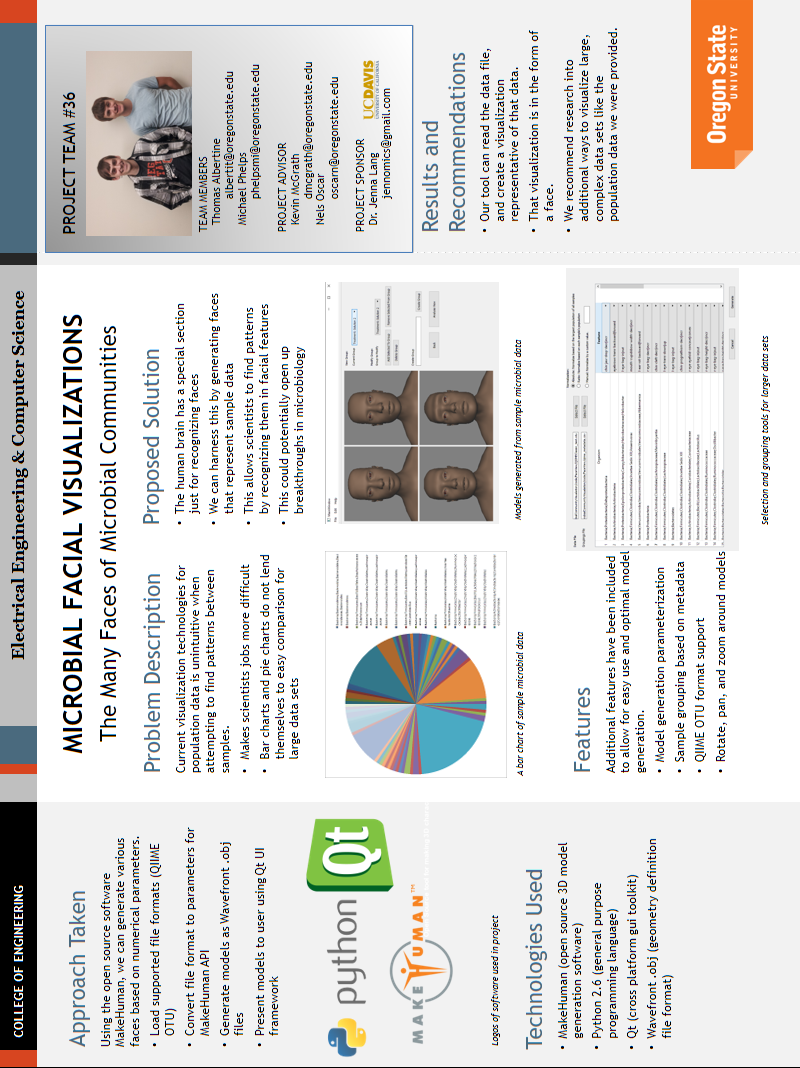
\includegraphics[height=\textheight]{Poster.png}
%	\caption{A flowchart representing the general structure of the project.}
%	\label{fig:structure}
%\end{figure}
\end{center}
\restoregeometry


\section{Project Documentation}
\subsection{How does the project work?}
\subsubsection{Structure}

There are five primary components of our application. They are the File Loader, the Model Generator Translator, the Model Generator, the Model Loader, and the Frontend. Figure \ref{fig:structure2} provides an overview of the relationships between the components.

 \begin{figure}[h]
	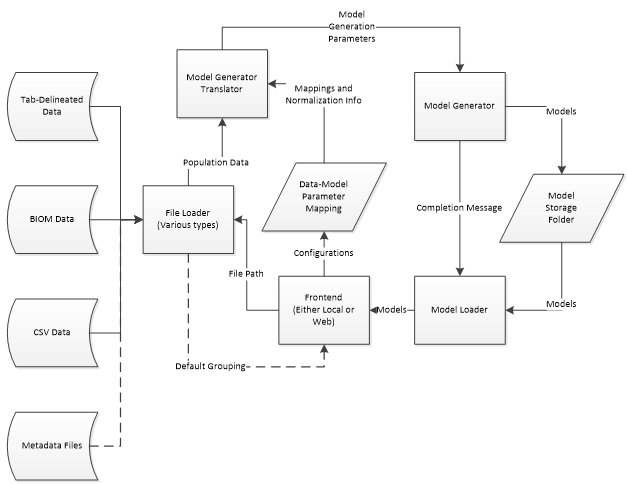
\includegraphics[width=\textwidth]{structure.PNG}
	\caption{A flowchart representing the general structure of the project.}
	\label{fig:structure2}
\end{figure}

As described in the figure, various formats of population data are loaded into the program through the File Loader. The File Loader splits the data file and metadata file into population data and sample groupings data, which are sent to the Model Generator Translator and Frontend respectively. From the Frontend, the user provides a mapping of model parameters (such as head shape, nose length, etc.) as well as information on how to normalize the data sent to the Model Generator Translator. The Model Generator Translator takes the mappings, population data, and normalization data and uses it to create parameters for the model generator. These parameters, which are simply pairs of model parameters with corresponding numbers between zero and 1, are sent to the Model Generator which uses them to customize a 3d model of a human. This model is saved in obj format in a designated folder. The Model generator can function as a standalone program, so when it finishes, the original program can stop waiting and begin loading those models. Those models are then presented to the user as the visualization.

\subsubsection{Theory of Operation}
Within each general component, there is still room for explanation.

The File Loader is composed of a registry object that contains several file loader objects. In the registry, each file loader object is associated with a file type (by file extension) in order to support multiple population data formats. Each can accept a population data file as well as an optional metadata file. When the file loader object is finished, it outputs a list of sample objects, as well as a list of group objects, which are simply lists of sample objects with some comparison functionality built in. The group objects are sent to the frontend so the user can select by group, or modify groups. The population data, on the other hand, is sent to the model generator so it chan be transformed into model generation parameters.

Before that however, the Data-Model Parameter Mappings and normalization data must be provided by the user. The user enters this data through the screen showed in Figure \ref{fig:loadingmockup2}. Each organism in the file can be associated with a model parameter from our selection of 138 parameters which we pull from the Model Generator on program startup. Of course, not every organism or model parameter needs to be associated with anything. In that case, no mapping entry is created for that organism or parameter. 

\begin{figure}[h]
	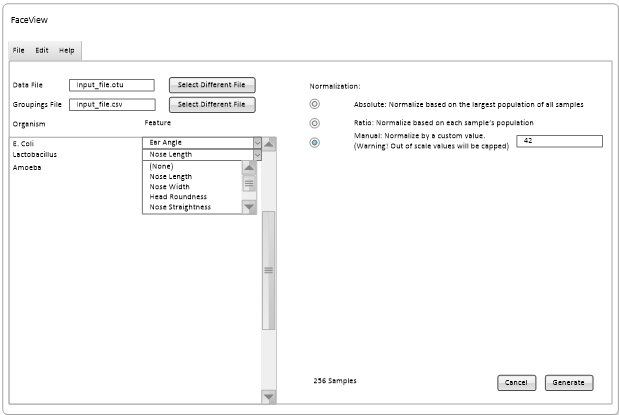
\includegraphics[width=\textwidth]{loadMenu.PNG}
	\caption{A mockup of the UI for loading a file containing three organisms and 256 samples, to be normalized with a maximum value of 42}
	\label{fig:loadingmockup2}
\end{figure}

Normalization information is fairly simple. There are three options. The first is that the data is normalized in absolute mode, which means that only the organism that has the highest population in the entire file will end up with a model parameter value of one, and all other parameters are scaled such that the proportions remain the same. This is good for comparing total populations of an organism between samples in a file. 

The second option is ratio mode. In this case, the organism with the highest population in each sample will have a model parameter value of one, scaling other organisms in the sample to maintain the proportions. This is good for comparing the ratios of a population between samples. 

The third option is manual mode. In this case, the value which all samples are divided by can be set by the user, allowing the user to compare samples with other samples of which they may have visualized before and taken screenshots. This mode runs the risk that the normalization value is not high enough. If that happens, the model parameters would come out to be greater than one, which isn't supported by our model generator. In this case, the value would be restricted to the range zero to one. We warn the user of this in the menu.

Once the data is loaded and the mappings and normalization information are chosen, the Model Generator translator can create the Model Generation Parameters. This process is relatively simple and done for each sample. For each organism in the sample, create a new entry. This entry's name should be the value that is mapped to the organism's name in the Data-Model Parameter Mapping. The value should be the population divided by the normalization value for the sample. Each sample's entries are delineated by a short message. The resulting parameter list is turned into a string and fed into the Model Generator's stdin.

The Model Generator was created to be a standalone program if necessary, in order to facilitate the web UI stretch goal. As such, it receives its input as console arguments and from stdin. It has two pieces of functionality. As mentioned before, the first function is to list the model parameters that it supports. That functionality is available by using a flag during invocation. Its main functionality however, is to read in the list of model parameters, and generate 3d human models based on those parameters. It does this by reading in the parameters, creating one parameter set for each group delineated by the message mentioned earlier. For each of these parameter sets, a MakeHuman human object is created. Each parameter is then applied to the human, and additional features (eyes, for example) are added before refreshing and updating the human. Then the human is exported to obj format and saved to a file in a designated folder, before resetting the human and moving on to the next parameter set.

When the Model Generation runs out of parameter sets, that program terminates, allowing the original program to continue. At that point the Model Loader is invoked, which loads the models and supports all of the necessary features of the Wavefront OBJ format. In terms of the geometry specification, it supports vertices, normal vectors, texture coordinates, faces, groups, and multiple materials. In terms of materials, it supports rgb colors for ambient, diffuse, and specular lighting components, as well as texture mapping. The Model Loader is closely tied to the OBJ viewer widget, which uses OpenGL to render the 3d models loaded here.

The OBJ viewer widget works with the Qt library. It performs initialization tasks in the initializeGL function, including loading and compiling shaders, and loading the data from the model objects into one vertex buffer object per group (using element array buffers for minimal duplication). For ease of use in the UI, it also provides functionality to create transformation matrices to rotate, scale, and translate models, as well as functions to generate those matrices from inputs that are easier to understand, such as rotating by some angle around an axis. At each draw cycle, for each group, updated uniform variables (such as those matrices) are rebound before calling glDrawElements to draw to the screen.

\begin{figure}[h]
	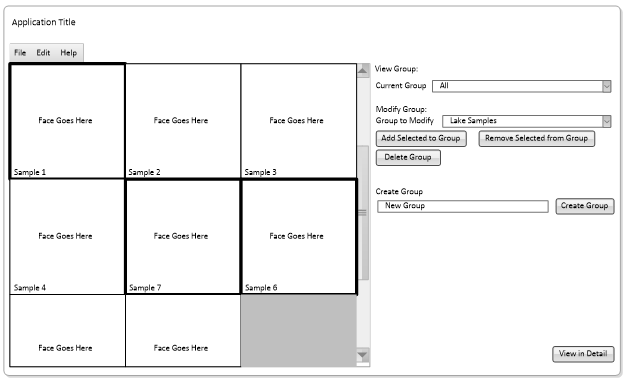
\includegraphics[width=\textwidth]{thumbnailMenu.PNG}
	\caption{A mockup of the thumbnail view.}
	\label{fig:thumbnail2}
\end{figure}

These models are associated with their original samples, so that they can be associated with the groups sent to the frontend initially. From there, they are shown to the user. Besides the file loading and parameter mapping screen, there are two additional screens. The first (Figure \ref{fig:thumbnail2}) is the thumbnail view, which allows user to quickly examine all of their samples and select some to analyze by clicking on them, as well as to select models by group.

The second screen is the analysis screen (Figure \ref{fig:analysis2}), which allows users to view the visualizations in more detail. Users can rotate the models to see the different features more clearly, and we provide buttons for commonly used camera positions. Specifically, we provide left and right side views, a front view, and a 3/4 view (directly looking at the model's left temple). Additionally, we provide a table containing the current mappings, so the user can easily see which organisms correspond to which features.

\begin{figure}[h]
	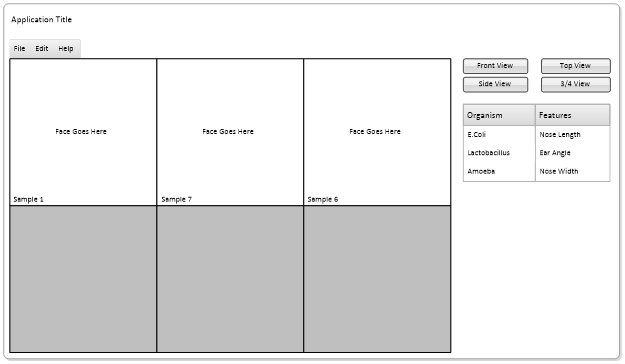
\includegraphics[width=\textwidth]{analysisMenu.PNG}
	\caption{A mockup of the analysis view.}
	\label{fig:analysis2}
\end{figure}

\subsection{Installation Instructions}
\label{sec:Installation Instructions}
As our project is written in Python, the program does not need installation itself, but there are some modules that you may have to install. In addition to standard modules packaged with Python, our project uses the following:

\begin{itemize}
	\item PyOpenGL
	\item Numpy
	\item Pillow
	\item PyQt4
\end{itemize}

PyOpenGL is a module that allows us to use the OpenGL graphics library to render the models. Numpy is a library that allows us to use lower level data structures for performance and to better interface with PyOpenGL. Pillow is a Python image library that we use to load textures. Specifically, we use it to load the texture on the eyes. Finally, PyQt4 is the library we use for our UI.

To install the first 3 modules is as simple as opening a command prompt and typeing ``pip install'' followed by the name of the module. Due to its license, PyQt4 is not available through Pip, so instead, you can use one of the installers found at \href{https://www.riverbankcomputing.com/software/pyqt/download}{riverbankcomputing.com}.

\subsection{How to Run}
\label{sec:How to Run}

After downloading our application, ther are a few options. If you have Python 2.7 associated with ``.py'' files, simply navigate to our project directory, then open the folder ``FaceView''. From there you can double click on ``main.py'' and the application should launch.

If you do not have Python 2.7 associated with ``.py'' files, you need to open a command prompt (or PowerShell) in that folder. Then run ``python main.py'', which should launch the application.

If it does not run, then it is possible that you do not have the correct version of Python installed, or you are using a different Python version by default.

\subsection{Additional Requirements}
Since our project is written in Python, and therefore requires Python 2.7 to run. Additionally, we require an OpenGL 2.0 or greater compatible graphics card for rendering.

Officially, we only support Windows. Unofficially however, there exist OS X versions of or substitutes for all the modules we use in our program as well.

\subsection{User Guide}
Hello and welcome to the FaceView Population Visualization Tool. Before we begin, please refer to sections \ref{sec:Installation Instructions} and \ref{sec:How to Run} to make sure that you are prepared to run this application.

Now that you have the application running, begin by clicking the button to select a data file. This allows you to choose which data file to visualize. For your convenience, we've included ``trivial.otu'' for demonstration purposes.

After selecting a data file, please click the button to select a metadata file, located just below the prevous button. This will allow you to select a metadata file containing sample groupings. We've included ``trivial.csv'' for your convenience, and debugging purposes.

After loading one of each file, the table should be populated with the organisms in your data file, on the left, and a drop down menu on the right. If you click the drop down menu, you should see a list of model parameters, by selecting one, you are associating that parameter with an organism in each sample. That is, a large population of that organism with make that feature more pronounced, whereas a small population would make it less pronounced. 

Please choose some associations now. We have noticed that parameters associated with the chin or head shape tend to be the most intuitive and the easiest to see and compare.

Now please take a moment to look at the upper right corner of the window. The normalization options scale your data so that the visualizations can show the whole picture. There are three options. ``Absolute'' normalizes your data in terms of the whole file. That is, every population count is scaled by the largest population in the file. That way, the relationship between the populations in the file are the same, but it is on a scale that our application can draw effectively. This mode is good for comparing the total population of an organism between multiple samples.

The second mode is ``Ratio'' mode, in which populations are scaled based on the largest population in the sample. This scheme is best for comparing the proportional makeup of a population, since the ratios within the sample are preserved.

The third normalization scheme is ``Manual'' in which you can set the normalization value. In this scheme, all of the populations are divided by the value you provide. For the purposes of this calculation, the final values must be between zero and one. Any values outside this range will be clamped to one of the edges, so be careful.

Now that all of the optoins are configured, please click the generate button, and the application will generate 3d models of human faces that represent your data. It may take a moment, so please be patient.

At this point, I'd like to point out that if you don't like your selection thus far, each page has a back button, which will allow you to return to the previous page with all of your settings maintained, so you can easily modify the parameters to fit your needs.

By the time the next window appears, the models will have finished generating and loading, and should be visible on your screen. At this point you can select them manually by clicking on them, or you can use the buttons on the right to select them by groups. If you had groups in your metadata file, you should have some groups in the drop down by default. In any case, can use those buttons to create groups, and samples to a group, remove samples from a group, or delete groups entirely (don't worry, the samples will remain). Please select some samples, and then click the button labelled ``Analysis View''

You should now see the analysis view. On the left, your selected samples should appear. You can click and drag them to rotate around the model to view the features you modified. On the right you should see several buttons at the top. These will move the camera to one of several common camera positions. Also on the right is a table containing the mapping between organisms and facial features that you created earlier.

\section{Learning New Technologies}

\subsection{Web Sites}

\subsubsection{Stack Overflow}
This answer may be the most obvious, but it was exceptionally helpful. If I searched for a question on Google, Stack Overflow was usually the first result. It's not a specialized resource, but it provides good advice and explanation on a wide variety of topics.

\url{http://stackoverflow.com/}

\subsubsection{Python Online Documentation}

Since our project was written in Python, it's obvious that the Python documentation would be useful. Again, it was more of a general resource, but still provided enough depth to get some good information.

\url{https://docs.python.org/2.7/}

\subsubsection{Qt 4.8 Documentation}
As we mentioned, our application is written using the PyQt4, which is a Python wrapper around the Qt UI library. Since the naming conventions were the same, we were able to read the Qt documentation to find out about the corresponding functionality in PyQt. As a bonus, the Qt documentation was searchable and easier to read than the official PyQt documentation.

\url{http://doc.qt.io/qt-4.8/}

\subsubsection{opengl-tutorial.org}
This site was a bit more specialized. It was a good refresher for how to work with OpenGL after not doing so for nearly a year. 

\url{http://www.opengl-tutorial.org/}

\subsubsection{QIIME Documentation}
This is the web site for the program that first used QIIME format, which we support. In the documentation, we found an explanation for the file format itself, which proved very helpful.

\url{http://qiime.org/documentation/index.html}

\section{Personal Learning}
\subsection{Thomas Albertine}
\subsubsection{Technical Information}
This project has been my first experience working with Qt. Admittedly, Michael did most of the UI work, but I had a hand in some of it as well. I did have some experience working with the Android SDK, which includes a UI framework, so I wasn't going in completely blind, but some features in Qt work differently than in Android. Besides that, all of the function and class names were different than Android's, but that goes without saying.

In the project, I had the opportunity to brush up on my OpenGL. As I mentioned before, it's been some time since I had a reason to do so, and I had forgotten how to set up vertex attribute arrays and element array buffers for example, even if I still remembered how they work conceptually. To tie this in with Qt, I had never done OpenGl with anything besides GLUT, so I also learned a bit about OpenGL contexts themselves and how to use the UI toolkit to get one.

Additionally, I've had the opportunity to learn of a few more \LaTeX packages. PgfGantt in particular was very helpful during this writeup. 

\subsubsection{Non-Technical Information}
I think the non-technical skill that I improved the most during this project was my ability to read someone else's code. I read other people's before (in particular, the Linux kernel in Operating Systems 2 and coworkers' code during my internship), but it was a drudgery and it took a long time to find anything. Perhaps it's the fact that the code for this project was in Python instead of C, but I didn't feel that is was as bad as before.

Other than that, I learned a bit about what was required for the kinds of documentation that we wrote. I understand that I was supposed to have learned that in Software Engineering, but at the time, we were so swamped with the project, unrelated papers, and tests that the actual documentation that is typically the focus of the class fell by the wayside. For that reason, I'm glad that I was able to make up the difference in Senior Design.

I also gained more experience in actually designing the project. Again this sounds like a Software Engineering topic, but in my class, only the three team leads got that opportunity. In Senior Design however, I personally had a lot more freedom with how the project worked, so I actually got to put the various design patterns into practice.

\subsubsection{Regarding Project Work}
Aside from where it intersects with the other categories, I don't think I've learned that much about project work itself in Senior Design. I don't fault the class, the format, or the instructor for that. I've just had a large number of projects in various other classes and in internships. That's not to say that I think I've learned everything I can from doing projects. It's just that, within the category project work alone, I don't think Senior Design is significantly different from what I've already done, except for the scale.

\subsubsection{Regarding Project Management}
The most important thing I learned about project management was how big a difference the client makes. I understand that as a developer, I won't always be able to pick which clients I work with, but I attribute a large part of our project's success to our client. We had a meeting in which we discussed requirements, which she provided. We wrote up a requirements document and althoguh She suggested one more at the time, she didn't change them at all throughout the year, and she was very understanding when some requirements needed to be adjusted for technical reasons. I attribute a large part of our success to our client's benevolence, especially considering some of the stories I've heard about other clients.

\subsubsection{Regarding Working in Teams}
The main thing I learned is that it's important to keep all the team members on the same page. The first time we had a discrepency regarding that caused me to panic and take over one of Michael's tasks. The second time led to us submitting the wrong version of one of the writeups. It doesn't really matter who's fault it is, because when comunication breaks down, it looks bad for both of us.

\subsubsection{What I Would Do Differently, If I Did It Again}
As I mentioned before, I think this project went surprisingly well. That said, there are a few places where we could have done better. As I also mentioned before, our communication was generally very good, but there were two major breaks in communication, that I would avoid were I to try again. 

There were, of course, things that were out of our hands. For example, in the original requirements document, we told our client that we could support 150 facial features, but we didn't yet know how to use MakeHuman to generate models, so we had to do so with the understanding that this number may have to change. When we found out, we spoke with our client and changed it to 138 features instead. That said, in an ideal world, I would have had time to figure out a more accurate number.

\subsection{Michael Phelps}
\subsubsection{Technical Information}
Prior to this project, I had incredibly minimal experience with writing programs in Python and no experience whatsoever on actually working on a full Python project. I had a bit of information from a some previous classes on coding in Python, but this is limited and this project ended up requiring a much more in depth knowledge of the language. The majority of my work on the project ended up being focused on the front-end. Having never developed any kind of UI for a program before, this ended up being a completely new skill for me to learn. Since we decided to use Qt for our interface, I ended up learning a great deal about the Qt libraries and how to properly develop with them. 

In addition to learning new coding skills, I also decided to work on this project entirely on my local windows machine which I had not done much before. Most of my development had previously been done on Unix-based systems. I was surprised to discover that developing on Windows and installing the necessary packages and libraries was not as simple as I expected it to be.

\subsubsection{Non-Technical Information}
One of the main skills which I learned during this project was developing the various types of technical documents that are needed for a software project. Previous classes did not really prepare me for the kind of technical writing that was needed in this course. It was especially educational having a great deal of feedback for all of the documents that we made.

\subsubsection{Communication}
One of the problems that I ran into when developing this project was not realizing that some parts of the code were using libraries that I did not have access to. I believe that this problem really came down to an innitial lack in communication, limiting the information I had on the commits being added to the code. I learned that it is important to keep up to date on communicating back and forth in order to ensure that everyone is using the proper libraries with the proper versions. 

\appendix[Essential Code Listings]
The following is an edited version of our code, removing uninteresting code (imports, tests, some functionality, etc.). The full code is available from our Github repository at \url{https://github.com/phelpsmi/MicrobialCommunityVisualation}.

\subsubsection{fvParser.py}
fvParser.py contains the parser registry, which works by associating each individual parser object with a file extension. When the file extension is provided, the registry knows which object to use, and we can extend the functionality by creating more parser objects.

\lstinputlisting{FaceView/fvParser.py}

\subsubsection{otuParser.py}
otuParser.py contains the parser object for the QIIME classic OTU format. It is an example of how a parser object can work.

\lstinputlisting{FaceView/otuParser.py}

\subsubsection{modelGeneratorTranslator.py}
modelGeneratorTranslator.py includes only the three functions for normalizing data. 

\lstinputlisting{FaceView/modelGeneratorTranslator.py}

\subsubsection{ModelGenerator.py}
This file includes functionality to invoke MakeHuman in order to either request a list of model parameters or to generate models themselves. If run by itself, this file becomes the application that generates the models. Otherwise, it is the library that invokes itself using the subprocess module. 

\lstinputlisting{FaceView/ModelGenerator.py}

\subsubsection{objModel.py}
This file contains the obj loading and mtl loading functionality. It supports a large part of the Wavefront obj specification. Specifically, it supports the features that MakeHuman uses in its generated obj files.

\lstinputlisting{FaceView/objviewer/objModel.py}


\appendix[Additional Content]

\end{document}
